\chapter{Program Structure}\label{program_structure}

\epigraphhead[30]{
\epigraph{\hspace*{-.1cm}\itshape``And my heart glows bright red under my filmy, translucent skin and they have to administer 10cc of JavaScript to get me to come back. (I respond well to toxins in the blood.) Man, that stuff will kick the peaches right out your gills!''}%
{---\_why, Why's (Poignant) Guide to Ruby}
}\index{why}\index{Poignant Guide}

In this chapter, we will start to do things that can actually be called \emph{programming}. We will expand our command of the JavaScript language beyond the nouns and sentence fragments we've seen so far, to the point where we can express meaningful prose.

\section{Expressions and statements}\index{grammar}\index{syntax!expression}\index{code!structure of}\index{grammar}\index{JavaScript!syntax}

In \hyperref[values]{Chapter 1}, we made values and applied operators to them to get new values. Creating values like this is the main substance of any JavaScript program. But that substance has to be framed in a larger structure to be useful. So that's what we'll cover next.\index{literal expression}\index{parentheses!expression}

A fragment of code that produces a value is called an \emph{\index{expression}expression}. Every value that is written literally (such as \lstinline`22` or \lstinline`"psychoanalysis"`) is an expression. An expression between parentheses is also an expression, as is a \index{binary operator}binary operator applied to two expressions or a \index{unary operator}unary operator applied to one.\index{nesting!of expressions}\index{human language}

This shows part of the beauty of a language-based interface. Expressions can contain other expressions in a way similar to how subsentences in human languages are nested—a subsentence can contain its own subsentences, and so on. This allows us to build expressions that describe arbitrarily complex computations.\index{statement}\index{semicolon}\index{program}

If an expression corresponds to a sentence fragment, a JavaScript \emph{statement} corresponds to a full sentence. A program is a list of statements.\index{syntax!statement}

The simplest kind of statement is an expression with a semicolon after it. This is a program:

\begin{lstlisting}
1;
!false;
\end{lstlisting}
\noindent

It is a useless program, though. An \index{expression}expression can be content to just produce a value, which can then be used by the enclosing code. A \index{statement}statement stands on its own, so it amounts to something only if it affects the world. It could display something on the screen—that counts as changing the world—or it could change the internal state of the machine in a way that will affect the statements that come after it. These changes are called \emph{\index{side effect}side effects}. The statements in the previous example just produce the values \lstinline`1` and \lstinline`true` and then immediately throw them away. This leaves no impression on the world at all. When you run this program, nothing observable happens.\index{programming style}\index{automatic semicolon insertion}\index{semicolon}

In some cases, JavaScript allows you to omit the semicolon at the end of a statement. In other cases, it has to be there, or the next \index{line}line will be treated as part of the same statement. The rules for when it can be safely omitted are somewhat complex and error-prone. So in this book, every statement that needs a semicolon will always get one. I recommend you do the same, at least until you've learned more about the subtleties of missing semicolons.

\section{Bindings}\index{variable|see{binding}}\index{syntax!statement}\index{binding!definition}\index{side effect}\index{memory!organization}\index{state!in!binding}

How does a program keep an internal state? How does it remember things? We have seen how to produce new values from old values, but this does not change the old values, and the new value has to be immediately used or it will dissipate again. To catch and hold values, JavaScript provides a thing called a \emph{binding}, or \emph{variable}:

\begin{lstlisting}
let caught = 5 * 5;
\end{lstlisting}
\noindent\index{let keyword}

That's a second kind of \index{statement}statement. The special word (\emph{\index{keyword}keyword}) \lstinline`let` indicates that this sentence is going to define a binding. It is followed by the name of the binding and, if we want to immediately give it a value, by an \lstinline`=` operator and an expression.

The previous statement creates a binding called \lstinline`caught` and uses it to grab hold of the number that is produced by multiplying 5 by 5.

After a binding has been defined, its name can be used as an \index{expression}expression. The value of such an expression is the value the binding currently holds. Here's an example:

\begin{lstlisting}
let ten = 10;
console.log(ten * ten);
// → 100
\end{lstlisting}
\noindent\index{= operator}\index{assignment}\index{binding!assignment}

When a binding points at a value, that does not mean it is tied to that value forever. The \lstinline`=` operator can be used at any time on existing bindings to disconnect them from their current value and have them point to a new one.

\begin{lstlisting}
let mood = "light";
console.log(mood);
// → light
mood = "dark";
console.log(mood);
// → dark
\end{lstlisting}
\noindent\index{binding!model of}\index{tentacle (analogy)}

You should imagine bindings as tentacles, rather than boxes. They do not \emph{contain} values; they \emph{grasp} them—two bindings can refer to the same value. A program can access only the values that it still has a reference to. When you need to remember something, you grow a tentacle to hold on to it or you reattach one of your existing tentacles to it.

Let's look at another example. To remember the number of dollars that Luigi still owes you, you create a binding. And then when he pays back \$35, you give this binding a new value.

\begin{lstlisting}
let luigisDebt = 140;
luigisDebt = luigisDebt - 35;
console.log(luigisDebt);
// → 105
\end{lstlisting}
\noindent\index{undefined}

When you define a binding without giving it a value, the tentacle has nothing to grasp, so it ends in thin air. If you ask for the value of an empty binding, you'll get the value \lstinline`undefined`.\index{let keyword}

A single \lstinline`let` statement may define multiple bindings. The definitions must be separated by commas.

\begin{lstlisting}
let one = 1, two = 2;
console.log(one + two);
// → 3
\end{lstlisting}
\noindent

The words \lstinline`var` and \lstinline`const` can also be used to create bindings, in a way similar to \lstinline`let`.

\begin{lstlisting}
var name = "Ayda";
const greeting = "Hello ";
console.log(greeting + name);
// → Hello Ayda
\end{lstlisting}
\noindent\index{var keyword}

The first, \lstinline`var` (short for ``variable''), is the way bindings were declared in pre-2015 JavaScript. I'll get back to the precise way it differs from \lstinline`let` in the \hyperref[functions]{next chapter}. For now, remember that it mostly does the same thing, but we'll rarely use it in this book because it has some confusing properties.\index{const keyword}\index{naming}

The word \lstinline`const` stands for \emph{\index{constant}constant}. It defines a constant binding, which points at the same value for as long as it lives. This is useful for bindings that give a name to a value so that you can easily refer to it later.

\section{Binding names}\index{underscore character}\index{dollar sign}\index{binding!naming}

Binding names can be any word. Digits can be part of binding names—\lstinline`catch22` is a valid name, for example—but the name must not start with a digit. A binding name may include dollar signs (\lstinline`$`) or underscores (\lstinline`_`) but no other punctuation or special characters.\index{syntax!identifier}\index{implements (reserved word)}\index{interface (reserved word)}\index{package (reserved word)}\index{private (reserved word)}\index{protected (reserved word)}\index{public (reserved word)}\index{static (reserved word)}\index{void operator}\index{yield (reserved word)}\index{enum (reserved word)}\index{reserved word}\index{binding!naming}

Words with a special meaning, such as \lstinline`let`, are \emph{\index{keyword}keywords}, and they may not be used as binding names. There are also a number of words that are ``reserved for use'' in \index{future}future versions of JavaScript, which also can't be used as binding names. The full list of keywords and reserved words is rather long.

\begin{lstlisting}
break case catch class const continue debugger default
delete do else enum export extends false finally for
function if implements import interface in instanceof let
new package private protected public return static super
switch this throw true try typeof var void while with yield
\end{lstlisting}
\noindent\index{syntax!error}

Don't worry about memorizing this list. When creating a binding produces an unexpected syntax error, see whether you're trying to define a reserved word.

\section{The environment}\index{standard environment}\index{browser!environment}

The collection of bindings and their values that exist at a given time is called the \emph{\index{environment}environment}. When a program starts up, this environment is not empty. It always contains bindings that are part of the language \index{standard}standard, and most of the time, it also has bindings that provide ways to interact with the surrounding system. For example, in a browser, there are functions to interact with the currently loaded website and to read \index{mouse}mouse and \index{keyboard}keyboard input.

\section{Functions}\index{application (of functions)|see{function!application}}\index{invoking (of functions)|see{function!application}}\index{calling (of functions)|see{function!application}}\index{output}\index{function}\index{function!application}\index{browser!environment}

A lot of the values provided in the default environment have the type \emph{\index{function}function}. A function is a piece of program wrapped in a value. Such values can be \emph{applied} in order to run the wrapped program. For example, in a browser environment, the binding \lstinline`prompt` holds a function that shows a little \index{dialog box}dialog box asking for user input. It is used like this:

\begin{lstlisting}
prompt("Enter passcode");
\end{lstlisting}
\noindent

\vskip 1.5ex
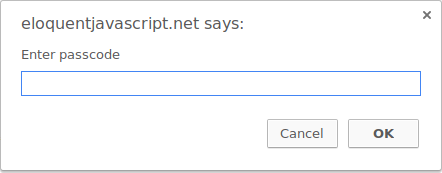
\includegraphics[width=8cm]{img/prompt.png}
\vskip 1.5ex\index{parameter}\index{function!application}\index{parentheses!arguments}

Executing a function is called \emph{invoking}, \emph{calling}, or \emph{applying} it. You can call a function by putting parentheses after an expression that produces a function value. Usually you'll directly use the name of the binding that holds the function. The values between the parentheses are given to the program inside the function. In the example, the \lstinline`prompt` function uses the string that we give it as the text to show in the dialog box. Values given to functions are called \emph{\index{argument}arguments}. Different functions might need a different number or different types of arguments.

The \lstinline`prompt` function isn't used much in modern web programming, mostly because you have no control over the way the resulting dialog looks, but can be helpful in toy programs and experiments.

\section{The console.log function}\index{JavaScript console}\index{developer tools}\index{Node.js}\index{console.log}\index{output}\index{browser!environment}

In the examples, I used \lstinline`console.log` to output values. Most JavaScript systems (including all modern web browsers and Node.js) provide a \lstinline`console.log` function that writes out its arguments to \emph{some} text output device. In browsers, the output lands in the \index{JavaScript
console}JavaScript
console. This part of the browser interface is hidden by default, but most browsers open it when you press F12 or, on a Mac, \textsc{command}-\textsc{option}-I. If that does not work, search through the menus for an item named Developer Tools or similar.\index{object!property}\index{property!access}

Though binding names cannot contain \index{period character}period characters, \lstinline`console.log` does have one. This is because \lstinline`console.log` isn't a simple binding. It is actually an expression that retrieves the \lstinline`log` property from the value held by the \lstinline`console` binding. We'll find out exactly what this means in \hyperref[data.properties]{Chapter 4}.

\label{program_structure.return_values}\section{Return values}\index{comparison!of numbers}\index{return value}\index{Math.max function}\index{maximum}

Showing a dialog box or writing text to the screen is a \emph{\index{side
effect}side
effect}. A lot of functions are useful because of the side effects they produce. Functions may also produce values, in which case they don't need to have a side effect to be useful. For example, the function \lstinline`Math.max` takes any amount of number arguments and gives back the greatest.

\begin{lstlisting}
console.log(Math.max(2, 4));
// → 4
\end{lstlisting}
\noindent\index{function!application}\index{minimum}\index{Math.min function}

When a function produces a value, it is said to \emph{return} that value. Anything that produces a value is an \index{expression}expression in JavaScript, which means function calls can be used within larger expressions. Here a call to \lstinline`Math.min`, which is the opposite of \lstinline`Math.max`, is used as part of a plus expression:

\begin{lstlisting}
console.log(Math.min(2, 4) + 100);
// → 102
\end{lstlisting}
\noindent

The \hyperref[functions]{next chapter} explains how to write your own functions.

\section{Control flow}\index{execution order}\index{program}\index{control flow}

When your program contains more than one \index{statement}statement, the statements are executed as if they are a story, from top to bottom. This example program has two statements. The first one asks the user for a number, and the second, which is executed after the first, shows the \index{square}square of that number.

\begin{lstlisting}
let theNumber = Number(prompt("Pick a number"));
console.log("Your number is the square root of " +
            theNumber * theNumber);
\end{lstlisting}
\noindent\index{number!conversion to}\index{type coercion}\index{Number function}\index{String function}\index{Boolean function}\index{Boolean!conversion to}

The function \lstinline`Number` converts a value to a number. We need that conversion because the result of \lstinline`prompt` is a string value, and we want a number. There are similar functions called \lstinline`String` and \lstinline`Boolean` that convert values to those types.

Here is the rather trivial schematic representation of straight-line control flow:

\vskip 1.5ex

\includegraphics[width=4cm]{img/generated/controlflow-straight.pdf}
\vskip 1.5ex

\section{Conditional execution}\index{Boolean}\index{control flow!conditional}

Not all programs are straight roads. We may, for example, want to create a branching road, where the program takes the proper branch based on the situation at hand. This is called \emph{\index{conditional
execution}conditional
execution}.

\vskip 1.5ex

\includegraphics[width=4cm]{img/generated/controlflow-if.pdf}
\vskip 1.5ex\index{syntax!statement}\index{Number function}\index{if keyword}

Conditional execution is created with the \lstinline`if` keyword in JavaScript. In the simple case, we want some code to be executed if, and only if, a certain condition holds. We might, for example, want to show the square of the input only if the input is actually a number.

\begin{lstlisting}
let theNumber = Number(prompt("Pick a number"));
if (!Number.isNaN(theNumber)) {
  console.log("Your number is the square root of " +
              theNumber * theNumber);
}
\end{lstlisting}
\noindent

With this modification, if you enter ``parrot'', no output is shown.\index{parentheses!statement}

The \lstinline`if` keyword executes or skips a statement depending on the value of a Boolean expression. The deciding expression is written after the keyword, between parentheses, followed by the statement to execute.\index{Number.isNaN function}

The \lstinline`Number.isNaN` function is a standard JavaScript function that returns \lstinline`true` only if the argument it is given is \lstinline`NaN`. The \lstinline`Number` function happens to return \lstinline`NaN` when you give it a string that doesn't represent a valid number. Thus, the condition translates to ``unless \lstinline`theNumber` is not-a-number, do this''.\index{grouping}\index{\{\} (block)}\index{braces!block}

The statement after the \lstinline`if` is wrapped in braces (\lstinline`{` and \lstinline`}`) in this example. The braces can be used to group any number of statements into a single statement, called a \emph{\index{block}block}. You could also have omitted them in this case, since they hold only a single statement, but to avoid having to think about whether they are needed, most JavaScript programmers use them in every wrapped statement like this. We'll mostly follow that convention in this book, except for the occasional one-liner.

\begin{lstlisting}
if (1 + 1 == 2) console.log("It's true");
// → It's true
\end{lstlisting}
\noindent\index{else keyword}

You often won't just have code that executes when a condition holds true, but also code that handles the other case. This alternate path is represented by the second arrow in the diagram. You can use the \lstinline`else` keyword, together with \lstinline`if`, to create two separate, alternative execution paths.

\begin{lstlisting}
let theNumber = Number(prompt("Pick a number"));
if (!Number.isNaN(theNumber)) {
  console.log("Your number is the square root of " +
              theNumber * theNumber);
} else {
  console.log("Hey. Why didn't you give me a number?");
}
\end{lstlisting}
\noindent\index{if keyword!chaining}

If you have more than two paths to choose from, you can ``chain'' multiple \lstinline`if`/\lstinline`else` pairs together. Here's an example:

\begin{lstlisting}
let num = Number(prompt("Pick a number"));

if (num < 10) {
  console.log("Small");
} else if (num < 100) {
  console.log("Medium");
} else {
  console.log("Large");
}
\end{lstlisting}
\noindent

The program will first check whether \lstinline`num` is less than 10. If it is, it chooses that branch, shows \lstinline`"Small"`, and is done. If it isn't, it takes the \lstinline`else` branch, which itself contains a second \lstinline`if`. If the second condition (\lstinline`< 100`) holds, that means the number is between 10 and 100, and \lstinline`"Medium"` is shown. If it doesn't, the second and last \lstinline`else` branch is chosen.

The schema for this program looks something like this:

\vskip 1.5ex

\includegraphics[width=4cm]{img/generated/controlflow-nested-if.pdf}
\vskip 1.5ex

\label{program_structure.loops}\section{while and do loops}

Consider a program that outputs all \index{even number}even numbers from 0 to 12. One way to write this is as follows:

\begin{lstlisting}
console.log(0);
console.log(2);
console.log(4);
console.log(6);
console.log(8);
console.log(10);
console.log(12);
\end{lstlisting}
\noindent\index{control flow!loop}

That works, but the idea of writing a program is to make something \emph{less} work, not more. If we needed all even numbers less than 1,000, this approach would be unworkable. What we need is a way to run a piece of code multiple times. This form of control flow is called a \emph{\index{loop}loop}.

\vskip 1.5ex

\includegraphics[width=4cm]{img/generated/controlflow-loop.pdf}
\vskip 1.5ex\index{syntax!statement}\index{counter variable}

Looping control flow allows us to go back to some point in the program where we were before and repeat it with our current program state. If we combine this with a binding that counts, we can do something like this:

\begin{lstlisting}
let number = 0;
while (number <= 12) {
  console.log(number);
  number = number + 2;
}
// → 0
// → 2
//   … etcetera
\end{lstlisting}
\noindent\index{while loop}\index{Boolean}\index{parentheses!statement}

A \index{statement}statement starting with the keyword \lstinline`while` creates a loop. The word \lstinline`while` is followed by an \index{expression}expression in parentheses and then a statement, much like \lstinline`if`. The loop keeps entering that statement as long as the expression produces a value that gives \lstinline`true` when converted to Boolean.\index{state!in!binding}\index{binding!as!state}

The \lstinline`number` binding demonstrates the way a \index{binding}binding can track the progress of a program. Every time the loop repeats, \lstinline`number` gets a value that is 2 more than its previous value. At the beginning of every repetition, it is compared with the number 12 to decide whether the program's work is finished.\index{exponentiation}

As an example that actually does something useful, we can now write a program that calculates and shows the value of 2\textsuperscript{10} (2 to the 10th power). We use two bindings: one to keep track of our result and one to count how often we have multiplied this result by 2. The loop tests whether the second binding has reached 10 yet and, if not, updates both bindings.

\begin{lstlisting}
let result = 1;
let counter = 0;
while (counter < 10) {
  result = result * 2;
  counter = counter + 1;
}
console.log(result);
// → 1024
\end{lstlisting}
\noindent

The counter could also have started at \lstinline`1` and checked for \lstinline`<= 10`, but for reasons that will become apparent in \hyperref[data.array_indexing]{Chapter 4}, it is a good idea to get used to counting from 0.\index{loop body}\index{do loop}\index{control flow!loop}

A \lstinline`do` loop is a control structure similar to a \lstinline`while` loop. It differs only on one point: a \lstinline`do` loop always executes its body at least once, and it starts testing whether it should stop only after that first execution. To reflect this, the test appears after the body of the loop.

\begin{lstlisting}
let yourName;
do {
  yourName = prompt("Who are you?");
} while (!yourName);
console.log(yourName);
\end{lstlisting}
\noindent\index{Boolean!conversion to}\index{"! operator}

This program will force you to enter a name. It will ask again and again until it gets something that is not an empty string. Applying the \lstinline`!` operator will convert a value to Boolean type before negating it, and all strings except \lstinline`""` convert to \lstinline`true`. This means the loop continues going round until you provide a non-empty name.

\section{Indenting Code}\index{code!structure of}\index{whitespace!indentation}\index{programming style}

In the examples, I've been adding spaces in front of statements that are part of some larger statement. These spaces are not required—the computer will accept the program just fine without them. In fact, even the \index{line}line breaks in programs are optional. You could write a program as a single long line if you felt like it.

The role of this \index{indentation}indentation inside \index{block}blocks is to make the structure of the code stand out. In code where new blocks are opened inside other blocks, it can become hard to see where one block ends and another begins. With proper indentation, the visual shape of a program corresponds to the shape of the blocks inside it. I like to use two spaces for every open block, but tastes differ—some people use four spaces, and some people use \index{tab character}tab characters. The important thing is that each new block adds the same amount of space.

\begin{lstlisting}
if (false != true) {
  console.log("That makes sense.");
  if (1 < 2) {
    console.log("No surprise there.");
  }
}
\end{lstlisting}
\noindent

Most code \index{editor}editor programs will help by automatically indenting new lines the proper amount.

\section{for loops}\index{syntax!statement}\index{while loop}\index{counter variable}

Many loops follow the pattern shown in the \lstinline`while` examples. First a ``counter'' binding is created to track the progress of the loop. Then comes a \lstinline`while` loop, usually with a test expression that checks whether the counter has reached its end value. At the end of the loop body, the counter is updated to track progress.\index{for loop}\index{loop}

Because this pattern is so common, JavaScript and similar languages provide a slightly shorter and more comprehensive form, the \lstinline`for` loop.

\begin{lstlisting}
for (let number = 0; number <= 12; number = number + 2) {
  console.log(number);
}
// → 0
// → 2
//   … etcetera
\end{lstlisting}
\noindent\index{control flow!loop}\index{state}

This program is exactly equivalent to the \hyperref[program_structure.loops]{earlier} even-number-printing example. The only change is that all the \index{statement}statements that are related to the ``state'' of the loop are grouped together after \lstinline`for`.\index{binding!as!state}\index{parentheses!statement}

The parentheses after a \lstinline`for` keyword must contain two \index{semicolon}semicolons. The part before the first semicolon \emph{initializes} the loop, usually by defining a binding. The second part is the \index{expression}expression that \emph{checks} whether the loop must continue. The final part \emph{updates} the state of the loop after every iteration. In most cases, this is shorter and clearer than a \lstinline`while` construct.\index{exponentiation}

This is the code that computes 2\textsuperscript{10} using \lstinline`for` instead of \lstinline`while`:

\begin{lstlisting}
let result = 1;
for (let counter = 0; counter < 10; counter = counter + 1) {
  result = result * 2;
}
console.log(result);
// → 1024
\end{lstlisting}
\noindent

\section{Breaking Out of a Loop}\index{loop!termination of}\index{break keyword}

Having the looping condition produce \lstinline`false` is not the only way a loop can finish. There is a special statement called \lstinline`break` that has the effect of immediately jumping out of the enclosing loop.

This program illustrates the \lstinline`break` statement. It finds the first number that is both greater than or equal to 20 and divisible by 7.

\begin{lstlisting}
for (let current = 20; ; current = current + 1) {
  if (current % 7 == 0) {
    console.log(current);
    break;
  }
}
// → 21
\end{lstlisting}
\noindent\index{remainder operator}\index{\% operator}

Using the remainder (\lstinline`%`) operator is an easy way to test whether a number is divisible by another number. If it is, the remainder of their division is zero.\index{for loop}

The \lstinline`for` construct in the example does not have a part that checks for the end of the loop. This means that the loop will never stop unless the \lstinline`break` statement inside is executed.

If you were to remove that \lstinline`break` statement or you accidentally write an end condition that always produces \lstinline`true`, your program would get stuck in an \emph{\index{infinite loop}infinite loop}. A program stuck in an infinite loop will never finish running, which is usually a bad thing.\index{continue keyword}

The \lstinline`continue` keyword is similar to \lstinline`break`, in that it influences the progress of a loop. When \lstinline`continue` is encountered in a loop body, control jumps out of the body and continues with the loop's next iteration.

\section{Updating bindings succinctly}\index{assignment}\index{+= operator}\index{-=@−= operator}\index{/= operator}\index{*= operator}\index{state!in!binding}\index{side effect}

Especially when looping, a program often needs to ``update'' a binding to hold a value based on that binding's previous value.

\begin{lstlisting}
counter = counter + 1;
\end{lstlisting}
\noindent

JavaScript provides a shortcut for this.

\begin{lstlisting}
counter += 1;
\end{lstlisting}
\noindent

Similar shortcuts work for many other operators, such as \lstinline`result *= 2` to double \lstinline`result` or \lstinline`counter -= 1` to count downward.

This allows us to shorten our counting example a little more.

\begin{lstlisting}
for (let number = 0; number <= 12; number += 2) {
  console.log(number);
}
\end{lstlisting}
\noindent\index{++ operator}\index{--@−− operator}

For \lstinline`counter += 1` and \lstinline`counter -= 1`, there are even shorter equivalents: \lstinline`counter++` and \lstinline`counter--`.

\section{Dispatching on a value with switch}\index{syntax!statement}\index{conditional execution}\index{dispatch}\index{if keyword!chaining}

It is not uncommon for code to look like this:

\begin{lstlisting}
if (x == "value1") action1();
else if (x == "value2") action2();
else if (x == "value3") action3();
else defaultAction();
\end{lstlisting}
\noindent\index{colon character}\index{switch keyword}

There is a construct called \lstinline`switch` that is intended to express such a ``dispatch'' in a more direct way. Unfortunately, the syntax JavaScript uses for this (which it inherited from the C\slash Java line of programming languages) is somewhat awkward—a chain of \lstinline`if` statements may look better. Here is an example:

\begin{lstlisting}
switch (prompt("What is the weather like?")) {
  case "rainy":
    console.log("Remember to bring an umbrella.");
    break;
  case "sunny":
    console.log("Dress lightly.");
  case "cloudy":
    console.log("Go outside.");
    break;
  default:
    console.log("Unknown weather type!");
    break;
}
\end{lstlisting}
\noindent\index{fallthrough}\index{break keyword}\index{case keyword}\index{default keyword}

You may put any number of \lstinline`case` labels inside the block opened by \lstinline`switch`. The program will start executing at the label that corresponds to the value that \lstinline`switch` was given, or at \lstinline`default` if no matching value is found. It will continue executing, even across other labels, until it reaches a \lstinline`break` statement. In some cases, such as the \lstinline`"sunny"` case in the example, this can be used to share some code between cases (it recommends going outside for both sunny and cloudy weather). But be careful—it is easy to forget such a \lstinline`break`, which will cause the program to execute code you do not want executed.

\section{Capitalization}\index{capitalization}\index{binding!naming}\index{whitespace!syntax}

Binding names may not contain spaces, yet it is often helpful to use multiple words to clearly describe what the binding represents. These are pretty much your choices for writing a binding name with several words in it:

\begin{lstlisting}
fuzzylittleturtle
fuzzy_little_turtle
FuzzyLittleTurtle
fuzzyLittleTurtle
\end{lstlisting}
\noindent\index{camel case}\index{programming style}\index{underscore character}

The first style can be hard to read. I rather like the look of the underscores, though that style is a little painful to type. The \index{standard}standard JavaScript functions, and most JavaScript programmers, follow the bottom style—they capitalize every word except the first. It is not hard to get used to little things like that, and code with mixed naming styles can be jarring to read, so we follow this \index{convention}convention.\index{Number function}\index{constructor}

In a few cases, such as the \lstinline`Number` function, the first letter of a binding is also capitalized. This was done to mark this function as a constructor. What a constructor is will become clear in \hyperref[object.constructors]{Chapter 6}. For now, the important thing is not to be bothered by this apparent lack of \index{consistency}consistency.

\section{Comments}\index{readability}

Often, raw code does not convey all the information you want a program to convey to human readers, or it conveys it in such a cryptic way that people might not understand it. At other times, you might just want to include some related thoughts as part of your program. This is what \emph{\index{comment}comments} are for.\index{slash character}\index{line comment}

A comment is a piece of text that is part of a program but is completely ignored by the computer. JavaScript has two ways of writing comments. To write a single-line comment, you can use two slash characters (\lstinline`//`) and then the comment text after it.

\begin{lstlisting}
let accountBalance = calculateBalance(account);
// It's a green hollow where a river sings
accountBalance.adjust();
// Madly catching white tatters in the grass.
let report = new Report();
// Where the sun on the proud mountain rings:
addToReport(accountBalance, report);
// It's a little valley, foaming like light in a glass.
\end{lstlisting}
\noindent\index{block comment}

A \lstinline`//` comment goes only to the end of the line. A section of text between \lstinline`/*` and \lstinline`*/` will be ignored in its entirety, regardless of whether it contains line breaks. This is useful for adding blocks of information about a file or a chunk of program.

\begin{lstlisting}
/*
  I first found this number scrawled on the back of an old notebook.
  Since then, it has often dropped by, showing up in phone numbers
  and the serial numbers of products that I've bought. It obviously
  likes me, so I've decided to keep it.
*/
const myNumber = 11213;
\end{lstlisting}
\noindent

\section{Summary}

You now know that a program is built out of statements, which themselves sometimes contain more statements. Statements tend to contain expressions, which themselves can be built out of smaller expressions.

Putting statements after one another gives you a program that is executed from top to bottom. You can introduce disturbances in the flow of control by using conditional (\lstinline`if`, \lstinline`else`, and \lstinline`switch`) and looping (\lstinline`while`, \lstinline`do`, and \lstinline`for`) statements.

Bindings can be used to file pieces of data under a name, and they are useful for tracking state in your program. The environment is the set of bindings that are defined. JavaScript systems always put a number of useful standard bindings into your environment.

Functions are special values that encapsulate a piece of program. You can invoke them by writing \lstinline`functionName(argument1, argument2)`. Such a function call is an expression and may produce a value.

\section{Exercises}\index{exercises}

If you are unsure how to test your solutions to the exercises, refer to the \hyperref[intro]{Introduction}.

Each exercise starts with a problem description. Read this description and try to solve the exercise. If you run into problems, consider reading the hints at the \hyperref[hints]{end of the book}. Full solutions to the exercises are not included in this book, but you can find them online at \href{https://eloquentjavascript.net/code#2}{\emph{https://eloquentjavascript.net\slash code}}. If you want to learn something from the exercises, I recommend looking at the solutions only after you've solved the exercise, or at least after you've attacked it long and hard enough to have a slight headache.

\subsection{Looping a triangle}\index{triangle (exercise)}

Write a \index{loop}loop that makes seven calls to \lstinline`console.log` to output the following triangle:

\begin{lstlisting}
#
##
###
####
#####
######
#######
\end{lstlisting}
\noindent\index{string!length}

It may be useful to know that you can find the length of a string by writing \lstinline`.length` after it.

\begin{lstlisting}
let abc = "abc";
console.log(abc.length);
// → 3
\end{lstlisting}
\noindent

\subsection{FizzBuzz}\index{FizzBuzz (exercise)}\index{loop}\index{conditional execution}

Write a program that uses \lstinline`console.log` to print all the numbers from 1 to 100, with two exceptions. For numbers divisible by 3, print \lstinline`"Fizz"` instead of the number, and for numbers divisible by 5 (and not 3), print \lstinline`"Buzz"` instead.

When you have that working, modify your program to print \lstinline`"FizzBuzz"` for numbers that are divisible by both 3 and 5 (and still print \lstinline`"Fizz"` or \lstinline`"Buzz"` for numbers divisible by only one of those).

(This is actually an \index{interview question}interview question that has been claimed to weed out a significant percentage of programmer candidates. So if you solved it, your labor market value just went up.)

\subsection{Chessboard}\index{chessboard (exercise)}\index{loop}\index{nesting!of loops}\index{newline character}

Write a program that creates a string that represents an 8×8 grid, using newline characters to separate lines. At each position of the grid there is either a space or a \textquotedbl{}\#\textquotedbl{} character. The characters should form a chessboard.

Passing this string to \lstinline`console.log` should show something like this:

\begin{lstlisting}
 # # # #
# # # # 
 # # # #
# # # # 
 # # # #
# # # # 
 # # # #
# # # #
\end{lstlisting}
\noindent

When you have a program that generates this pattern, define a binding \lstinline`size = 8` and change the program so that it works for any \lstinline`size`, outputting a grid of the given width and height.
